\subsection{\textbf{Generalization.}}
Here the test performance of SVEA is compared to 5 recent state-of-the-art methods for image-based RL on the \texttt{color\_hard} and \texttt{video\_easy} benchmarks from DMControl-GB, as well as the extremely challenging DistractingCS benchmark, where camera pose, background, and colors are continually changing throughout an episode. Here \textit{conv} and \textit{overlay} augmentations are used and we report additional results on the \texttt{video\_hard} benchmark. SVEA outperforms all methods considered in $\mathbf{12}$ out of $\mathbf{15}$ instances on DMControl-GB, and at a lower computational cost than CURL, PAD, and SODA that all learn auxiliary tasks. On DistractingCS, we observe that SVEA improves generalization by $\mathbf{42\%}$ at low intensity, and its generalization degrades significantly slower than DrQ for high intensities. While generalization depends on the particular choice of data augmentation and test environments, this is an encouraging result considering that SVEA enables efficient policy learning with stronger augmentations than previous methods.


\subsection{\textbf{Test Environments}}
Figure \ref{fig:test-env-visualization} provides visualizations for each of the two generalization benchmarks, DMControl Generalization Benchmark and Distracting Control Suite, used in our experiments. Agents are trained in a fixed training environment with no visual variation, and are expected to generalize to novel environments of varying difficulty and factors of variation. The \texttt{color\_hard}, \texttt{video\_easy}, and \texttt{video\_hard} benchmarks are from DMControl Generalization Benchmark, and we further provide samples from the Distracting Control Suite (DistractingCS) benchmark for intensities $I=\{0.1, 0.2, 0.5\}$. 
While methods are evaluated on a larger set of intensities, we here provide samples deemed representative of the intensity scale. We note that the DistractingCS benchmark has been modified to account for action repeat (frame-skip). Dynamically changing the environment at each simulation step makes the benchmark disproportionally harder for tasks that use a large action repeat, e.g. \textit{Cartpole} tasks. Therefore, we choose to modify the DistractingCS benchmark and instead update the distractors every second simulation step, corresponding to the lowest action repeat used (2, in \textit{Finger, spin}). This change affects both SVEA and baselines equally. Figure \ref{fig:dmc-dcs-individual} shows generalization results on DistractingCS for each task individually. We find that the difficulty of DistractingCS varies greatly between tasks, but SVEA consistently outperforms DrQ in terms of generalization across all intensities and tasks.

\begin{figure}
    \centering
    \begin{subfigure}[b]{0.48\textwidth}
        \centering
        
\includegraphics[width=\textwidth]{figures/visualizations/obs_env.png}
        \caption{Training environment (walker).}
        \vspace{0.1in}
    \end{subfigure}
    \begin{subfigure}[b]{0.48\textwidth}
        \centering
        
\includegraphics[width=\textwidth]{figures/visualizations/obs_cartpole_env.png}
        \caption{Training environment (cartpole).}
        \vspace{0.1in}
    \end{subfigure}
    \begin{subfigure}[b]{0.48\textwidth}
        \centering
        
\includegraphics[width=\textwidth]{figures/visualizations/obs_env_color_hard.png}
        \caption{\texttt{color\_hard} environment (walker).}
        \vspace{0.1in}
    \end{subfigure}
    \begin{subfigure}[b]{0.48\textwidth}
        \centering
        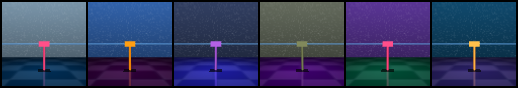
\includegraphics[width=\textwidth]{figures/visualizations/obs_cartpole_env_color_hard.png}
        \caption{\texttt{color\_hard} environment (cartpole).}
        \vspace{0.1in}
    \end{subfigure}
    \begin{subfigure}[b]{0.48\textwidth}
        \centering
        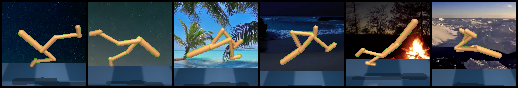
\includegraphics[width=\textwidth]{figures/visualizations/obs_env_video_easy.png}
        \caption{\texttt{video\_easy} environment (walker).}
        \vspace{0.1in}
    \end{subfigure}
    \begin{subfigure}[b]{0.48\textwidth}
        \centering
        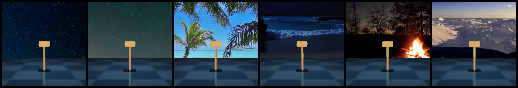
\includegraphics[width=\textwidth]{figures/visualizations/obs_cartpole_env_video_easy.png}
        \caption{\texttt{video\_easy} environment (cartpole).}
        \vspace{0.1in}
    \end{subfigure}
    \begin{subfigure}[b]{0.48\textwidth}
        \centering
        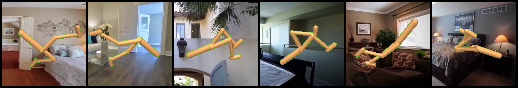
\includegraphics[width=\textwidth]{figures/visualizations/obs_env_video_hard.png}
        \caption{\texttt{video\_hard} environment (walker).}
        \vspace{0.1in}
    \end{subfigure}
    \begin{subfigure}[b]{0.48\textwidth}
        \centering
        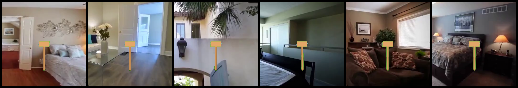
\includegraphics[width=\textwidth]{figures/visualizations/obs_cartpole_env_video_hard.png}
        \caption{\texttt{video\_hard} environment (cartpole).}
        \vspace{0.1in}
    \end{subfigure}
    \begin{subfigure}[b]{0.48\textwidth}
        \centering
        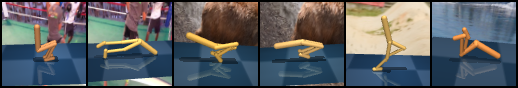
\includegraphics[width=\textwidth]{figures/visualizations/obs_env_dcs_easy.png}
        \caption{DistractingCS for intensity $0.1$ (walker).}
        \vspace{0.1in}
    \end{subfigure}
    \begin{subfigure}[b]{0.48\textwidth}
        \centering
        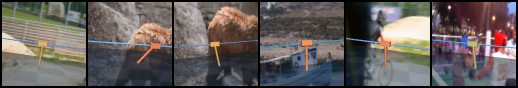
\includegraphics[width=\textwidth]{figures/visualizations/obs_cartpole_env_dcs_easy.png}
        \caption{DistractingCS for intensity $0.1$ (cartpole).}
        \vspace{0.1in}
    \end{subfigure}
    \begin{subfigure}[b]{0.48\textwidth}
        \centering
        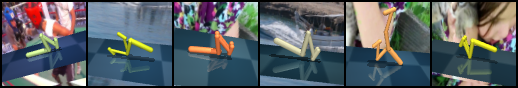
\includegraphics[width=\textwidth]{figures/visualizations/obs_env_dcs_medium.png}
        \caption{DistractingCS for intensity $0.2$ (walker).}
        \vspace{0.1in}
    \end{subfigure}
    \begin{subfigure}[b]{0.48\textwidth}
        \centering
        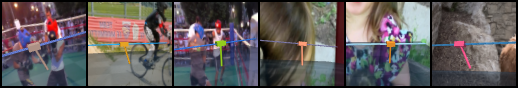
\includegraphics[width=\textwidth]{figures/visualizations/obs_cartpole_env_dcs_medium.png}
        \caption{DistractingCS for intensity $0.2$ (cartpole).}
        \vspace{0.1in}
    \end{subfigure}
    \begin{subfigure}[b]{0.48\textwidth}
        \centering
        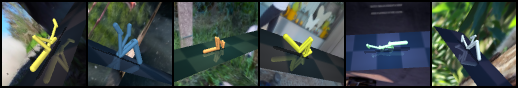
\includegraphics[width=\textwidth]{figures/visualizations/obs_env_dcs_extreme.png}
        \caption{DistractingCS for intensity $0.5$ (walker).}
        \vspace{0.1in}
    \end{subfigure}
    \begin{subfigure}[b]{0.48\textwidth}
        \centering
        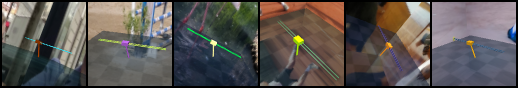
\includegraphics[width=\textwidth]{figures/visualizations/obs_cartpole_env_dcs_extreme.png}
        \caption{DistractingCS for intensity $0.5$ (cartpole).}
        \vspace{0.1in}
    \end{subfigure}
    \vspace{-0.1in}
    \caption{\textbf{Test environments}. Samples from each of the two generalization benchmarks, DMControl Generalization Benchmark and Distracting Control Suite, considered in this study. In our experiments, agents are trained in a fixed training environment with no visual variation, and are expected to generalize to novel environments of varying difficulty and factors of variation.}
    \label{fig:test-env-visualization}
    \vspace{-0.15in}
\end{figure}

\begin{figure}
    \centering
    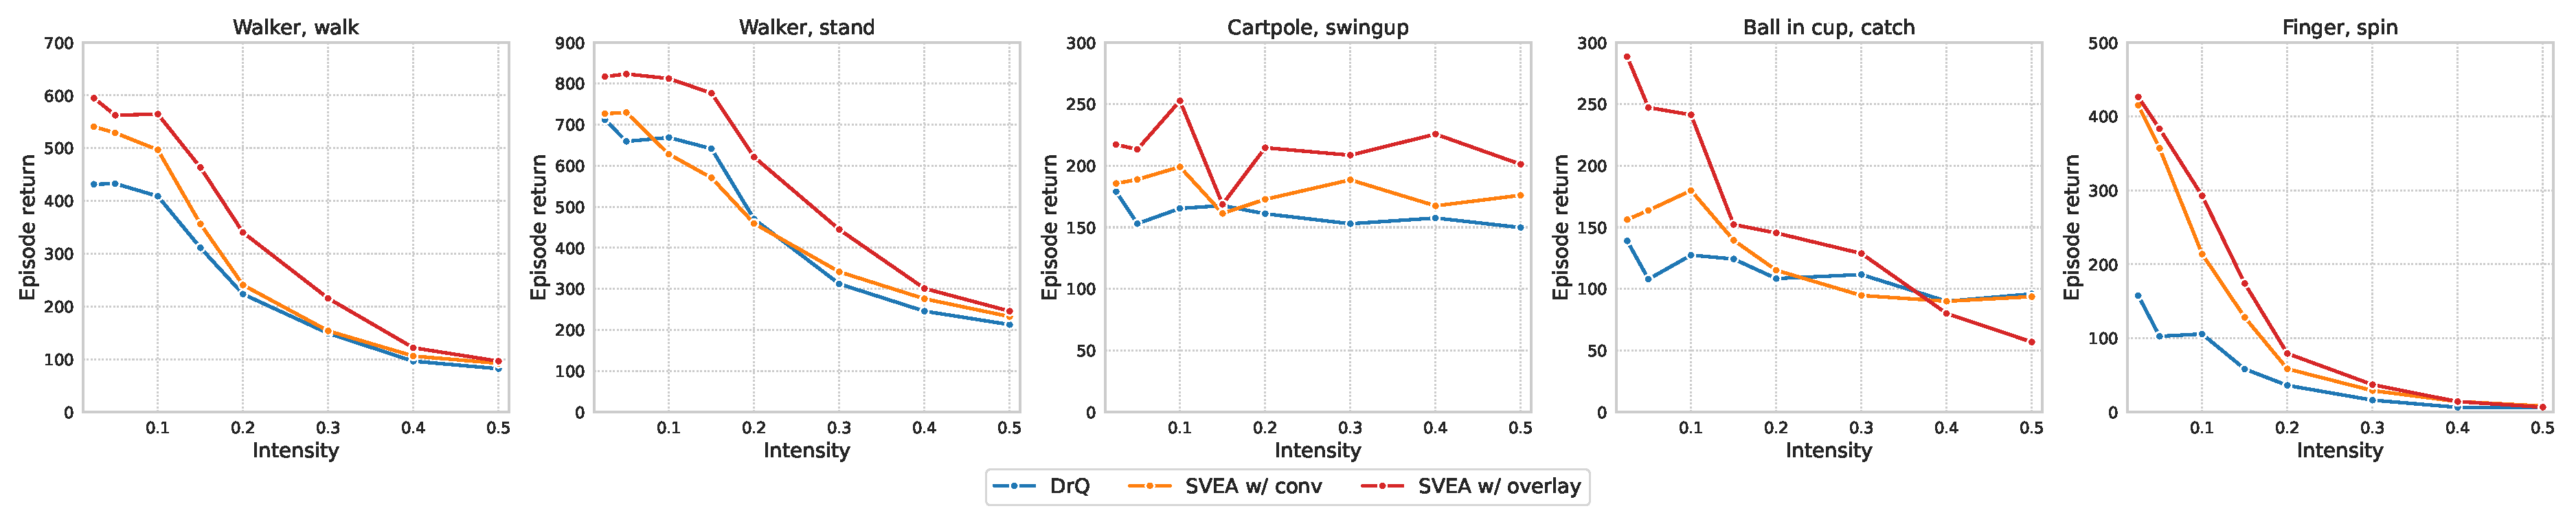
\includegraphics[width=\textwidth]{figures/dcs_individual.pdf}
    \vspace{-0.2in}
    \caption{\textbf{DistractingCS.} Episode return as a function of randomization intensity, for each of the 5 tasks from DMControl-GB (using ConvNets). Mean of 5 seeds. We find that the difficulty of DistractingCS varies greatly between tasks, but SVEA consistently outperforms DrQ in terms of generalization across all intensities and tasks, except for \textit{Ball in cup, catch} at the highest intensity.}
    \label{fig:dmc-dcs-individual}
    \vspace{-0.05in}
\end{figure}